\documentclass[]{spie}  %>>> use for US letter paper
%\documentclass[a4paper]{spie}  %>>> use this instead for A4 paper
%\documentclass[nocompress]{spie}  %>>> to avoid compression of citations

\renewcommand{\baselinestretch}{1.0} % Change to 1.65 for double spacing

\def\procspie{Proc.\ SPIE} % Proceedings of the SPIE

\usepackage{amsmath,amsfonts,amssymb}
\usepackage{graphicx}
\usepackage[colorlinks=true, allcolors=blue]{hyperref}

\title{LSST Data Management Software Development Practices and Tools}

\author[a]{Tim~Jenness}
\author[a]{Frossie~Economou}
\author[b]{Krzysztof~Findeisen}
\author[c]{Fabio~Hernandez}
\author[a]{Josh~Hoblitt}
\author[d]{Kian-Tat~Lim}
\author[d]{Fritz~Mueller}
\author[a]{William~O'Mullane}
\author[b]{Russell~Owen}
\author[e]{Stephen~R~Pietrowicz}
\author[f]{Pim~Schellart}
\author[a]{Jonathan~Sick}
\author[a]{Adam~Thornton}

\affil[a]{LSST Project Office, 950 N.\ Cherry Avenue, Tucson, AZ 85719, USA}
\affil[b]{University of Washington, Dept. of Astronomy, Box 351580, Seattle, WA 98195, USA}
\affil[c]{CNRS, CC-IN2P3, 21 avenue Pierre de Coubertin, CS70202, 69627 Villeurbanne cedex, France}
\affil[d]{SLAC National Accelerator Laboratory, 2575 Sand Hill Rd, Menlo Park, CA 94025, USA}
\affil[e]{NCSA, University of Illinois at Urbana-Champaign, 1205 W. Clark St. Urbana, IL 61801}
\affil[f]{Department of Astrophysical Sciences, Princeton University, Princeton, NJ 08544}


\authorinfo{Further author information: (Send correspondence to T.J.)\\T.J.: E-mail: tjenness@lsst.org,\\  W.O'M: E-mail: womullan@lsst.org}

% Option to view page numbers
\pagestyle{empty} % change to \pagestyle{plain} for page numbers
\setcounter{page}{1} % Set start page numbering at e.g. 301

\begin{document}
\maketitle

\begin{abstract}
The Large Synoptic Survey Telescope (LSST) is an 8.4m optical survey telescope being constructed on Cerro Pach\'on in Chile.
The data management system being developed must be able to process the nightly alert data, 20,000 expected transient alerts per minute, in near real time, and construct annual data releases at the petabyte scale.
The development team consists of more than 70 people working in six different sites across the US developing an integrated set of software to meet the LSST requirements.
In this paper we discuss our agile software development methodology and our API and developer decision making process.
We also discuss the software tools that we use for continuous integration and deployment.
\end{abstract}

% Include a list of keywords after the abstract
\keywords{}


\section{INTRODUCTION}

The Data Management System (DMS)\cite{2015arXiv151207914J} for the Large Synoptic Survey Telescope (LSST) \cite{2008arXiv0805.2366I} has been under development since at least 2004\cite{2004AAS...20510811A}.
During that time a number of technologies have been adopted and our development practices have evolved as we transitioned from the research and development phase to construction.
The Data Management (DM) team is distributed, with representation from Princeton University, the University of Washington, the National Center for Supercomputing Applications at Urbana-Champaign, IPAC in Pasadena, the LSST Project Office in Tucson, and the SLAC National Accelerator Laboratory near Stanford University; along with some external contributions from CC-IN2P3 in Lyon, France.
As a uniform survey, LSST is highly dependent on its Data Management System, which, like the telescope and camera, has requirements that have been at or beyond the state of the art of the time.
Unlike many science projects, even large ones, from the beginning LSST was recognized as needing a substantial software effort, and significant portions of both the design and development and the construction budgets have been devoted to that effort.
As a result, LSST has been able to hire full-time software engineering staff, including not only developers but also developer support staff.
Founding and growing the LSST Data Management team has thus been like creating a start-up software company.
Developers with experience in software engineering, not just scientific programming, were sought, several with experience in industry.
Best practices and tools used by open-source companies were adopted.
Evolution, not only of the code base but also of the development process itself, was embraced; developers were empowered to make changes.
Given the distributed team, it is important that comunication channels are open and easy to use and that our tools evolve as community standards evolve.
Being agile enough to be able to migrate from one tool to another during the lifetime of a project is key when the software, processes, and people, change over what will be a 25 year period once the 10-year survey completes.
For example, over the years we have migrated the codebase from Subversion to git (\S\ref{sec:subversion}); we have switched instant messaging from HipChat to Slack (\S\ref{sec:slack}); we have migrated continuous integration from Buildbot on our own hosts to Jenkins running in the cloud (\S\ref{sec:jenkins}); and we have moved documentation standards from Doxygen to Sphinx (\S\ref{sec:sphinx_tooling}).

In the following sections we describe the current development practices for LSST DM.

\section{Agile Development}\label{sec:agile}

LSST data management follows a long term plan with six month cycles. The  development approach falls in the rather  broad {\emph Agile} methodology. It is also beholden to organizations such as NSF which require a more traditional approach to project development such as the Earned Value Management System (EVMS).
We have presented this from both  the ESA and LSST perspective in SPIE previously  \cite{2014SPIE.9150E..1EG}.
In 2016  we presented a more complete approach for LSST to the problem of Agile in the earned value world \cite{2016SPIE.9911E..0NK}, here we provide just a brief update on that paper concentrating more on the Agile aspects.


\subsection{Management}
The Project Management Guide \cite{DMTN-020} provides  comprehensive details on the mechanisms underpinning LSST Data Management’s approach to project management, the reader is referred to to that document for gory details as required.
Each institution in the DM team is typically
responsible for 1 or more Level 2 WBS elements, and each institution has a Technical/Control Account Manager
(T/CAM) responsible for planning, estimating, monitoring and EVM reporting for that Level 2 WBS element.
The detailed management plan is in LDM-294\cite{LDM-294}.

\subsection{Basic Assumptions}
The Project assumes that a full-time individual works for a total of
1,800 hours per year: this figure is \emph{after} all vacations, sick
leave, etc are taken into account. Staff appointed to ``developer''
positions are expected to devote this effort directly to LSST.

Appointment as a {\emph scientist} includes a 20\% personal research time
allowance. That is, scientists are expected to devote 1,440 hours per
year to LSST, and the remainder of their time to personal research.

Our base assumption is that 30\% of an individual's LSST time (i.e. 540 hours/year for a developer, 432 hours/year for a scientist) are devoted to overhead for regular meetings\footnote{``Meetings'' include, for example, scheduled weekly team meetings, stand-ups, etc.; major conferences or project meetings involving preparation, travel time, etc. should be scheduled in advance and allocated Story Points}, ad-hoc discussions and other interruptions.
This is similar to the standard {\emph Agile} discount, however in the earned value world that must be accounted for and it is considered Level of Effort (LOE)


\subsection{Long Term Planning}
\label{sec:long-term-plan}

The plan for the duration of construction is embodied in:

\begin{enumerate}
\item
  A series of \emph{planning packages}, which describe major pieces of
  technical work. Planning packages are associated with concrete, albeit
  high-level, deliverables (in the shape of milestones), and have
  specific resource loads (staff assignments), start dates, and
  durations. The entire DM system is covered by around 100 of these
  planning packages.
\item
  \emph{Milestones} represent the delivery or availability of specific
  functionality. Each planning package culminates in a milestone, and
  may contain other milestones describing intermediate results.
\end{enumerate}

Planning packages are defined at the fourth level of the Work Breakdown Structure (WBS).

All WBS elements are related to the set of Data Management Products embodied in the System Design \cite{LDM-148} a high level summary of which is given in
Figure \ref{fig:prods}. Each product has a product owner to guide the agile development, this is frequently one of the Data Management Scientists.

\begin{figure}[htbp]
        \begin{center}
                 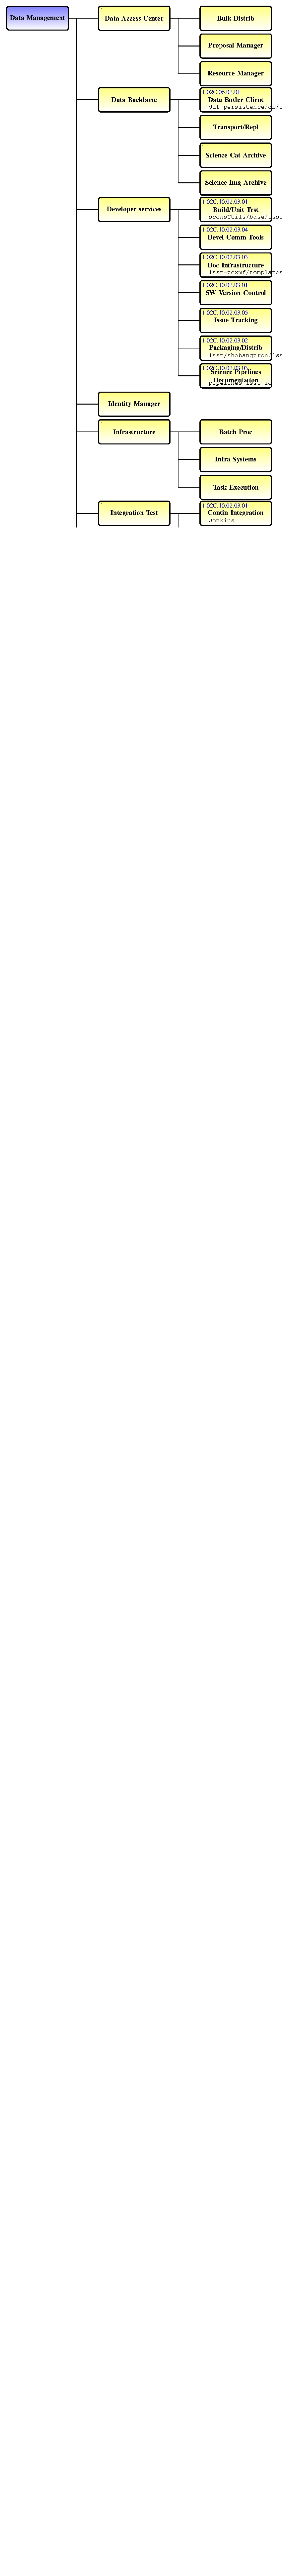
\includegraphics[height=10cm]{ProductTree}
                 \caption{DM product tree. \label{fig:prods} There are over 200 products in the full tree, this diagram shows a truncated form of the product tree to convey an idea of the products.
         }

         \end{center}
 \end{figure}

During the cycle planning process  effort is drawn from the budget embodied in the planning packages to generate the cycle plan, described in terms of epics in Jira.
Each epic itself has a particular budget.
This budget is subtracted from that available in the planning package at the point when the epic is defined.
Team members then add specific stories to these epics.

The Jira system is synchronized with the Primavera project management tool every three months using in-house tools.

In order for the DM system to reach its science goals, new algorithmic or engineering approaches must sometimes be researched.
It is appropriate to budget time for this research work in planning packages and they result in epics of defined length (rather than specific  deliverable).
Areas where successful delivery of the DM system is dependent on speculative research are a source of risk: where possible, the plan  also provides for a fallback option to be taken when research objectives are not achieved.
This may also lead to an entry in the risk register.


Some work is {\emph emergent}: we can predict in advance that it will be necessary, but we cannot
predict exactly what form it will take. The typical example of this is fixing bugs: we can reasonably
assume that bugs will be discovered in the codebase and will need to be addressed,
but we cannot predict in advance what those bugs will be.
We included this in the schedule by defining a {\emph bucket} epic in which stories can be created
when necessary during the course of a cycle.

\subsection{Sprinting} \label{sec:spront} \label{sec:jira_ticket}
The broad plan (to 2022)  laid out in planning packages.
For a  given  cycle (six months)   more detail is put in the form of epics which  are shared across the teams in a face to face meeting a little ahead of the start of cycle.  The team then start to populate the epics with stories (both of which are Jira tickets)  which are at an appropriate level for day to day planning.
Within the cycle we follow monthly sprints with the usual agile steps:
\begin{enumerate}
\item {\bf Preparation:} Stories for the sprint are chosen and distributed to team members according to available points. This is usually a local team meeting.
\item {\bf Execution:} As the cycle progresses daily standups are used to catch blockers and clarify stories. At the higher level there are two T/CAM standups each week on Tuesday and Friday to raise issues across team boundaries.
\item {\bf Review:} At cycle end a retrospective should be conducted.
\end{enumerate}

We use Jira's
\href{https://www.atlassian.com/software/jira/agile}{Agile} capabilities
to manage our sprints. Each technical manager is responsible for
defining and maintaining their own agile board. The board may be
configured for either
\href{https://en.wikipedia.org/wiki/Scrum_(software_development)}{Scrum}
or \href{https://en.wikipedia.org/wiki/Kanban_(development)}{Kanban}
style work as appropriate.

\subsection{Reporting }
DM produces a mandatory written monthly report for NSF/DOE in which each team reports on progress and issues. A new addition to this report since last year is to clearly track the state of milestones which have been met or delayed.
As the previous SPIE paper \cite{2016SPIE.9911E..0NK} pointed out the Primavera system outputs standard project metrics on variance and budget.
Though this is reasonable  for reporting hardware based activities it does not report well on Agile progress unless there are well defined deliverables.
In 2017 we have undertaken to lay out a set of test driven milestones to show progress in Data Management. These milestones are completed by execution of tests laid out in a test specification tying them to requirements, resulting in a test report.

\section{Model-Based Systems Engineering}

LSST uses Model-Based Systems Engineering\cite{2014SPIE.9150E..0MC}, with designs, requirements, and behavior described using the SysML language and stored within a database-backed tool, initially Enterprise Architect and now MagicDraw.
MagicDraw permits communication between teams through a unified model of the system.
It also allows for relatively easy maintenance of the requirements at all levels of the system as well as traceability between requirements and the system components that satisfy them.

Within the SysML language, there are specialized diagram types.
The Requirement Diagram documents requirements and their relationships.
Block Definition Diagrams highlighting interfaces and Internal Block Diagrams highlighting component breakdowns explicate the design of the system.
Activity Diagrams, Sequence Diagrams, State Machine Diagrams, and Use Case Diagrams show the system's intended behavior.
The MagicDraw tool allows these behavioral diagrams to be executed in a simulation mode to verify that the behavior is complete and correct.
All of this information is useful for the verification process.
Test cases are developed from requirements and behavior.

\subsection{Requirements}

Requirements are written using a combination of a formal specification, which uses verbs such as ``shall'' and ``will'' in a stylized manner, along with a description that explains the context and interpretation of the requirement.
Constraints are added to the requirement that document values of parameters used within the specification, along with their descriptions and units.
Each requirement is given a unique identifier generated based on its containing document and a monotonically-increasing sequence number.
This requirement id allows requirements to be safely referred to and linked together even if the containing document is reorganized or if a requirement is deleted or replaced by another.
Requirements document organization into sections is handled by grouping requirements into SysML packages.
Numbers prefixed to the titles of the packages and the requirements within them allow them to be sorted into a human-meaningful order.
These numbers are sequential within a containing package, not hierarchical, making renumbering and reorganization easier.
Requirements documents are generated using one of two custom macros, one for Microsoft Word documents and another for LaTeX documents.
The document generation macros sort the elements within packages and strip off the sequential prefix numbers, allowing the word processing tools to create the hierarchical section and requirement title numbers.
When LaTeX is used, the generated files are stored in git repositories and then follow the standard DM documentation release process.

\subsection{Requirements Documents}

Five levels of requirements documents are applicable to Data Management.
At the highest level, the LSST Science Requirements Document (SRD)\cite{LPM-17} sets out the overall scientific goals of the project in prose.
The LSST System Requirements\cite{LSE-29} are the project's formal response to the SRD, setting minimum, design, and ``stretch'' goals for requirement parameters.
The Observatory System Specifications\cite{LSE-30} documents requirements and budgets based on a high-level design, in particular partitioning the LSST system into Telescope \& Site, Camera, Data Management, and Education \& Public Outreach subsystems.
At this level, the Data Products Definition Document\cite{LSE-163} provides a full specification of the data products to be delivered by the LSST system.
The Data Management System Requirements (DMSR)\cite{LSE-61} are the flowdown to DM specifically.
At the same level as the DMSR, Interface Control Documents (ICDs) specify the relationships between the different subsystems.
Finally, within the DM system, component requirements documents are used where appropriate to constrain designs and provide for internal verification.

\subsection{Flowdown}

One of the excellent features of MagicDraw is the ability to rapidly document the flowdown of requirements.
Using a table with higher-level requirements on one side and lower-level requirements on the other, the ``refines'' relationship between the latter and the former can be created by merely toggling an arrow within appropriate table cells.
Unfortunately, it is more difficult to use the SysML ``copy'' relationship in cases where the lower-level requirement happens to be identical to the higher-level one.
It has been necessary to manually copy the requirement text (and generate a new requirement id, of course).

Since system components are also present in the MagicDraw model, the tool also helps with recording which requirements apply to each component, and, conversely, which components are needed to satisfy each requirement.

\subsection{Conclusion}

Ultimately, SysML and MagicDraw have been most useful for systems engineering purposes at the LSST system level, rather than within the Data Management system itself.
While the tool is fully capable of recording component designs in diagrammatic language, adoption has been somewhat difficult; developers tend to prefer to work directly on code.
In its place, more limited diagrams are produced using other tools such as OmniGraffle, Gliffy (particularly with the Confluence plugin), LaTeX, Archi, and \href{http://websequencediagrams.com}{websequencediagrams.com}.

\input{software}
\input{comms}
\input{docs}
\section{Decision Making Process}

During the research and development phase of the project, DM used a formal process for approving all changes to the DM system.
The SAT consisted of scientists and system architecture representatives and had regular meetings to discuss matters arising.
As the team size expanded into construction we realized that as the number of decisions to be made grew, fewer decisions were being made. (did we suffer from bikeshedding so I can cite that original story?)

We realized that there were two distinct classes of changes being discussed by the SAT.
On the one hand there were discussions relating to changes in the baseline design, requirements, budget, and sizing model, and the SAT membership was optimized to discuss these issues.
The other type of request related to requests from developers for modification to APIs, changes to compilers or build environemts, and changes to the coding style.
These latter issues generate debate from the people most directly affected by them and delays of weeks whilst a SAT meeting was convened, combined with the developers feeling they were not part of the deicsion making, led to much frustration.

[show Jira RFC workflow here?]

In 20?? we decided to change our approach to the latter process.
DM developers have to be familiar with Jira and we developed a Jira workflow for ``Request for Comments'' (RFCs).
RFCs were designed to empower individual developers to propose decisions.
Emphasis is placed on the developer being responsible for any fall out from a change.
If they propose an API change, they are agreeing that they will fix any breakage in other DM code; if they are proposing a change to the style guide they will make the change to the style guide.
When an RFC is submitted it enters the \emph{Proposed} state and the proposal is mailed to the DM developer list and an announcement is made on the main DM Slack channel.
For changes that are expected to have no real impact outside of a single package, a due date of 3 days is acceptable.
For changes that might result in significant debate, for example adding a new package to be supported by DM or changing an API used by many packages, the proposer is advised to give at least a week and possibly two weeks for debate.
Any one can comment on the RFC and when consensus is reached the RFC can be \emph{Adopted} by the proposer.
If consensus could not be reached the proposer has the option of withdrawing the RFC completely, adding more time, or flagging the RFC to the Change Control Board for more formal decision making.
On adoption, an RFC must be associated with actual work by filing tickets in DM Jira and connecting them with an ``is triggering'' relationship.
The DM Systems Engineer is tasked with looking at RFCs on a weekly basis to ensure that proposed RFCs are not languishing and that implemented RFCs are correctly marked as such.
The \emph{Implemented} state is recognized by scanning all the \emph{Adopted} RFCs and seeing that all triggered work has been completed.

The RFC process has been extremely successful with N RFCs filed since 201? and M implemented.
We have found that some RFCs are filed asking for changes that the proposer feels are a good change to make but which they themselves are not going to be repsonsible for implementing.
These are sometimes a very good idea but since there is no lead implementer, RFCs like this depend on T/CAMs picking up the work and scheduling it as part of their normal planning process.

\subsection{Change Control Board}

The LSST has a project level Change Control Board (CCB) for managing evolution of budgets, requirements and subsystem interfaces.
The LSST CCB meets regularly with formal meetings each month and weekly video calls.
The CCB process itself is mediated by a bespoke Drupal web app written early in the life of the project; this can lead to confusion when new people are asked to use the system and we would like to switch to Jira, if only that it would be one less tool to use and we could easily link work tickets to LSST Change Requests (LCRs).
Currently, there is no relationship between the LCR number and the URL and this is one of the main sources of friction with the system when seen from outside the CCB.
We do use Jira for work directly resulting from a CCB investigation, or for noting issues with project level change-controlled documentation that may need to be addressed when the person does not necessarily have a formal request prepared.

Inside DM we have our own formal CCB that has evolved over the years from the SAT to something we called the Technical Control Team (TCT) but which has now been reorganized as the DM CCB.
The DM CCB is chaired by the DM Systems Engineer and has representation from senior members of each DM team as well as the DM Project Manager and DM Subsystem Scientist.
DM CCB uses the same RFC process as described above, but issues to be discussed by the TCT are immediately submitted into the \emph{Flagged} state.
This is mainly used to discuss changes to the baseline documents and is also used to give formal DM approval to changes that DM are requesting to be made in project level documentation.
When deemed necessary some RFCs may require a video meeting to allow more direct discussion.

\section{Continuous Integration}

\subsection{Jenkins}
\label{sec:jenkins}

\subsubsection{Why Jenkins?}

The initial ``Continuous Integration'' system used for pre-merge testing of
science pipeline code was buildbotFOOTNOTE:URL-https://buildbot.net/.  While it
was able to accomplish the basic task of building branches from a git repo,
there were a number of drawbacks.
% \footnote{WRT the state of buildbot in 2014, the project appears to have made some improvements since that time}
A few of the issues were: the UI was spartan and difficult to navigate, no
integration with 3rd party authentication systems requiring manual management
of user accounts, bare-bones ``out of the box'' functionality without a useful
selection of publicly available plugins, and DM internal concern as to the long
term viability as there appeared be relatively few public/open source users
relative to competing CI/CD systems.

% should this be broken into a \item list?
After evaluating several potential CI/CD systems as a replacement,
JenkinsFOOTNOTE:URL-https://jenkins.io/ was selected for numerous reasons,
including: an open source core, it could be self hosted (the wall-clock build
time and memory requirements exceeded the limits of many of the commercial
hosted CI options, at that time), it offered an improved UI over buildbot,
there was a pre-existing plugin to use github
oauthFOOTNOTE:URL-https://plugins.jenkins.io/github-oauth, a healthy extension
ecosystem with many useful plugins, apparent popularity with self-hosted
open source projects, and an active core project.

\subsubsection{Configuration + Deployment}

The Jenkins core and various plugins need to be version managed and configured.
Although there is currently a major effort underway to add native
``configuration by
code''FOOTNOTE:URL-https://github.com/jenkinsci/configuration-as-code-plugin to
the jenkins core, this is not yet considered production ready and did not exist
at the time DM was transitioning away from buildbot.

PuppetFOOTNOTE:URL-https://puppet.com/ was selected as a configuration
management tool as, at that time, it had the most sophisticated jenkins
management abilities among the CM tools surveyed via the
\texttt{puppet-jenkins}FOOTNOTE:URL-https://github.com/voxpupuli/puppet-jenkins
module.  Non-trivial improvements have been contributed by DM staff to this
module
FOOTNOTE:URL-https://puppet.com/presentations/puppet-vs-jenkins-tale-types-and-providers
in order to make it more suitable for managing a jenkins deployment.

Configuration of Jenkins jobs is handled via the
\texttt{job-dsl}FOOTNOTE:URL-https://plugins.jenkins.io/job-dsl plugin.  This
enables a \texttt{groovy}FOOTNOTE:url-http://www.groovy-lang.org/ based DSL and a special job type that
will ``seed'' jenkins jobs from a git repository that contains \texttt{job-dsl}
script(s).  The seed job itself is maintained as \texttt{xml} that is manually
installed by puppet.  The result is that all jobs configuration is managed via
a SCM and no manual configuration via the jenkins UI is required to
add/delete/change or stand up a testing environment.

% should any of the jenkins related repos be mentioned?
% the production jenkins deployment is not publically accessible

% add discussion of jenkins pipeline

\subsubsection{Evolving Usage}

Over time, usage of jenkins has evolved from being used solely for pre-merge
``CI'' testing to automation of number of common tasks.  Among various sundry
tasks, it is being used to build docker images, update local software mirrors,
schedule regular backup.  Perhaps most notably, it is being used to a drive a
`Continuous Deployment'' workflow for completely automated nightly and weekly
release/publication of science pipelines codes(\ref{sec:scipipe-deploy}).

\subsection{Travis-CI}
\label{sec:travis-ci}

Travis for simpler items (yaml file validation, flake8 tests)

\input{cd}
\section{Conclusion}

The LSST Data Management Team consists of more than one hundred people spread across multiple locations.
In this paper we have described our current developer processes and explained how they have evolved over time and how we foresee them evolving in the future.
The LSST Data Management software development has been ongoing for at least 14 years and we expect that our processes will continue to evolve, based on experience and new technologies, as we transition from construction to operations through to the end of the survey in 2032.


\acknowledgments % equivalent to \section*{ACKNOWLEDGMENTS}

We thank all the people who have contributed to the discussions on tooling and process over the year.s
This material is based upon work supported in part by the National Science Foundation through Cooperative Agreement 1258333 managed by the Association of Universities for Research in Astronomy (AURA), and the Department of Energy under Contract No.\ DE-AC02-76SF00515 with the SLAC National Accelerator Laboratory.
Additional LSST funding comes from private donations, grants to universities, and in-kind support from LSSTC Institutional Members.

% References
\bibliography{spie-10707-10} % bibliography data
\bibliographystyle{spiebib} % makes bibtex use spiebib.bst

\end{document}
